\chapter{Revisão Bibliográfica}
\label{chap:conceitos}

Neste capítulo, serão apresentados os conceitos necessários para a compreensão do desenvolvimento deste trabalho, abordando os estudos relacionados ao monitoramento de sinais eletrocardiográficos (ECG) e as tecnologias de comunicação sem fio de baixo consumo, com ênfase na rede LoRaWAN.

\section{Trabalhos Relacionados}
\label{sec:trabalhosRelacionados}

O monitoramento remoto de sinais vitais, especialmente o \acs{ECG}, tem ganhado destaque na área da saúde devido à necessidade de acompanhamento contínuo de pacientes, principalmente em regiões com acesso limitado a serviços médicos especializados. A tecnologia LoRaWAN tem se mostrado uma solução promissora nesse contexto, oferecendo comunicação de longo alcance com baixo consumo de energia.

\subsection{Monitoramento Remoto de Sinais Vitais}
% - Falar dos artigos que fazem monitoramento de ECG, sinais vitais via IoT, etc.
O trabalho de \cite{7814958} propõe o desenvolvimento de uma aplicação IOT para transmissão de dados de mídia de sinal de \acs{ECG}. Foi desenvolvido um sistema que pode ser acessado simultaneamente via internet para o monitoramento dos sinais vitais coletados. O sistema consiste em um circuito analógico personalizado para captura de \acs{ECG} com eletrodos conectados conforme o triângulo de \textit{Einthoven}, um amplificador de biopotencial, filtros passa-alta (0,05 Hz) e \textit{butterworth} passa-baixa (40 Hz). O microcontrolador utilizado foi o ATmega328 para processamento dos sinais analógicos em digitais e transmissão via \textit{ZigBee}. Neste trabalho foi registrado captura dos sinais de ECG em 20 pacientes simultaneamente sem apresentar inconsistências nas transmissões.

O estudo de \cite{9920379} propõe uma solução inovadora para o monitoramento remoto em tempo real do status cardíaco de pacientes, utilizando sensores ECG e comunicação via LoRa 915 MHz em uma rede IoT. O ECG, essencial para detectar condições cardíacas como arritmias, é transmitido por meio da tecnologia LoRa. Os dados do ECG são recebidos pela plataforma ThingSpeak, permitindo que médicos e pacientes monitorem a saúde cardíaca em tempo real, independentemente da localização. O estudo também avalia o desempenho do LoRa em condições de sinal variável, especialmente em áreas densamente povoadas, analisando parâmetros como perda de pacotes, intensidade de sinal e taxa de erro. Os resultados demonstram a viabilidade e a eficácia da tecnologia para o monitoramento remoto e acessível da saúde cardíaca. Para a implementação, foram utilizados o módulo LoRa 915 MHz, o Dragino LoRa 915 MHz Gateway, o Arduino Uno e o módulo ECG AD8232.

No trabalho de \cite{8934622}, foi implementado um protótipo de monitoramento de ECG baseado em IoT, que se destacou como uma solução eficiente e de baixo custo, apresentando uma precisão de 80\% nas capturas dos sinais. O dispositivo utiliza a tecnologia de comunicação Wi-Fi, aliado a uma placa microcontroladora Arduino UNO para a captura dos sinais de ECG, com o sensor AD8232 conectado a ela. O Raspberry Pi foi empregado como plataforma de processamento dos dados, permitindo a análise em tempo real dos sinais de ECG. Além disso, foi desenvolvida uma interface gráfica acessível via web e aplicativos móveis, proporcionando aos usuários a visualização e monitoramento contínuo dos dados de saúde do paciente.

Voltado ao acompanhamento de pacientes fora do ambiente hospitalar, o sistema m-GreenCARDIO, proposto por \cite{mGreen}, integra a aquisição de \acs{ECG} a um sistema embarcado de baixo consumo com recursos de telemedicina, permitindo o registro contínuo da atividade cardíaca e a transmissão dos dados para acompanhamento clínico remoto. O trabalho enfatiza a importância de soluções portáteis que liberem o paciente das restrições do monitoramento hospitalar convencional, sem prejuízo da qualidade do sinal adquirido.

Em uma perspectiva voltada à equidade no acesso à saúde, \cite{dispLowCost} apresentam um arcabouço (\textit{framework}) de monitoramento cardíaco remoto de baixo custo concebido para regiões rurais. A solução combina um dispositivo vestível de aquisição de \acs{ECG} a uma arquitetura de \textit{m-health}, priorizando a transmissão eficiente dos dados em cenários de conectividade limitada — um desafio recorrente em localidades afastadas dos grandes centros médicos. Os autores destacam que o custo reduzido e a autonomia energética são fatores determinantes para a adoção dessas tecnologias em larga escala.

Em síntese, os trabalhos analisados convergem quanto à viabilidade técnica do monitoramento remoto de \acs{ECG} baseado em IoT, mas evidenciam um compromisso recorrente entre a tecnologia de comunicação adotada e os requisitos de alcance, consumo energético e taxa de dados. Enquanto soluções baseadas em Wi-Fi e ZigBee privilegiam a taxa de transmissão em detrimento do alcance e da autonomia, as abordagens emergentes baseadas em LoRa buscam justamente o oposto, abrindo espaço para o monitoramento em áreas extensas e com infraestrutura limitada, contexto no qual se insere este trabalho.


\subsection{Detecção Embarcada de Anomalias no ECG}
\label{sec:deteccaoEmbarcada}

Diferentemente dos trabalhos anteriores, centrados na aquisição e na transmissão do sinal, \citeay{moraesFirmwareECG} concentraram-se no processamento e na detecção automática de anomalias diretamente no dispositivo. Os autores desenvolveram um \textit{firmware} para o monitor multiparâmetros MP3.5, executado em um microcontrolador ESP32-S3, capaz de identificar, em tempo real, cinco anomalias associadas a alterações nos intervalos R-R do \acs{ECG}: taquicardia, bradicardia, arritmia, bloqueio e parada sinusais. A detecção dos picos R empregou o método da operação de diferenças (DOM, \textit{Difference Operation Method}), baseado na diferenciação do sinal, na filtragem passa-baixas e no pareamento de máximos e mínimos locais para localizar o complexo QRS; a partir dos picos detectados, os intervalos R-R foram analisados estatisticamente para a classificação das anomalias. O processamento foi realizado sobre segmentos de 30~s, e a validação, conduzida com a base de dados MIT-BIH e com sinais simulados acrescidos de ruído controlado, alcançou taxa de acerto de 99,92\% na detecção dos picos R e de 99,67\% na identificação das anomalias.

Esse \textit{firmware} constitui a base do algoritmo de detecção embarcada adotado nesta dissertação: seu código-fonte foi \textbf{cedido pelos autores} e aqui reutilizado, não constituindo, portanto, contribuição original deste trabalho. A opção pelo reúso, em vez da reimplementação de um detector, decorre de o método já haver sido validado — 99,92\% na detecção dos picos R e 99,67\% na identificação das anomalias — e de o foco desta pesquisa recair sobre a aquisição, o processamento na borda e a \textbf{transmissão} do \acs{ECG} em rede \textit{LoRaWAN}. Enquanto o sistema original foi concebido para um monitor multiparâmetros com processamento local, o presente trabalho parte do mesmo detector e o integra a uma arquitetura de transmissão de longo alcance por \textit{LoRaWAN}, com o posterior encaminhamento dos eventos para a nuvem e para um aplicativo móvel — aspecto não contemplado no trabalho de origem, e que constitui uma das contribuições desta pesquisa. Os detalhes da adaptação realizada para a plataforma adotada são apresentados na Seção~\ref{sec:deteccaoBorda}.

% TODO (ao receber o trabalho completo do Claudinei): completar os dados de publicação
% da entrada moraesFirmwareECG no main.bib; se pertinente, citar Yeh e Wang (método DOM
% original) e outros trabalhos correlatos de detecção embarcada que o usuário fornecer.


\subsection{Tecnologias de Comunicação Sem Fio Aplicadas ao Monitoramento de ECG}
% - Trabalhos comparando BLE, Wi-Fi, LoRa para ECG

Nesta subseção são apresentadas e comparadas três das principais tecnologias utilizadas nesse contexto: Wi-Fi, ZigBee e Bluetooth Low Energy (BLE), com ênfase em suas aplicações, vantagens e limitações no monitoramento de sinais de \acs{ECG}.


\subsubsection{Wi-Fi}

A evolução das tecnologias sem fio tem desempenhado um papel fundamental no desenvolvimento de sistemas de monitoramento remoto de sinais fisiológicos, com destaque para os sinais eletrocardiográficos (\acs{ECG}), que requerem baixa latência, confiabilidade na transmissão e eficiência energética. Entre essas tecnologias, o Wi-Fi (IEEE 802.11) configura-se como uma solução amplamente difundida em ambientes clínicos e domiciliares, por permitir altas taxas de transmissão (atingindo centenas de Mbps), o que o torna adequado para o envio de sinais de \acs{ECG} em tempo real, com elevada resolução temporal. No entanto, apesar dessa vantagem em termos de largura de banda, o consumo energético relativamente elevado dos módulos Wi-Fi pode ser um entrave em aplicações voltadas a dispositivos médicos portáteis ou vestíveis, os quais exigem longas autonomias operacionais. Nesses casos, são necessárias baterias de maior capacidade ou a adoção de estratégias como duty cycling e compressão de dados, a fim de prolongar a duração do sistema em operação (\citeay{SHEBIAHAMMED201365}).

\subsubsection{ZigBee}

Outra alternativa de destaque é o ZigBee (baseado na especificação IEEE 802.15.4), frequentemente utilizada em redes de sensores sem fio (Wireless Sensor Networks – WSNs) e redes pessoais sem fio (\textit{Wireless Personal Area Networks} – WPANs). O ZigBee apresenta como principais vantagens a baixa potência de operação, suporte à topologia em malha, e capacidade de escalabilidade para múltiplos dispositivos, sendo ideal para monitoramento simultâneo de vários pacientes em um mesmo ambiente (\citeay{4426313}). Embora sua taxa de transmissão (250 kbps) seja inferior à do Wi-Fi, é suficiente para transmitir sinais \acs{ECG} com amostragens típicas de 250 Hz a 500 Hz, após filtragem e quantização adequadas (\citeay{4745439}).

O uso do ZigBee em sistemas embarcados também favorece a miniaturização e o custo reduzido dos nós sensores. Contudo, por utilizar banda de 2.4 GHz e ter alcance limitado (cerca de 10 a 100 metros), pode sofrer interferências em ambientes com múltiplas redes sem fio, o que requer planejamento de canal e controle de qualidade de serviço (QoS) para aplicações críticas como telecardiologia (\citeay{gia2014customizing}).

\subsubsection{BLE}

No contexto de dispositivos médicos portáteis e da conectividade com smartphones, o Bluetooth Low Energy (BLE), introduzido a partir da especificação Bluetooth 4.0, consolidou-se como uma tecnologia predominante em aplicações biomédicas. O BLE é altamente eficiente em termos energéticos, permitindo que sensores operem por dias ou até semanas com uma pequena célula de lítio, uma característica essencial para dispositivos de \acs{ECG} vestíveis e de uso contínuo. Com taxa de transmissão de até 1 Mbps e baixa latência, o BLE é adequado para o envio contínuo de dados de sinais eletrocardiográficos para smartphones, os quais atuam como gateways para aplicações clínicas e sistemas em nuvem (\citeay{TOUATI2013124}).

Essa abordagem foi validada por \citeauthor{ecgBLE} (\citeyear{ecgBLE}), que desenvolveram um dispositivo eletrônico de baixo custo e reduzido consumo energético, projetado para transmitir segmentos de 30 segundos de \acs{ECG} a cada hora, com tempo de envio inferior a 2 segundos por transmissão. O sistema apresentou autonomia estimada superior a 16 dias, mantendo compatibilidade com um monitor multiparamétrico portátil e viabilidade de encapsulamento em formato compacto. A presença nativa do BLE em dispositivos móveis modernos facilita a adoção dessa tecnologia e permite sua integração eficiente com sistemas de monitoramento baseados em nuvem. Contudo, a literatura aponta que limitações como o número reduzido de conexões simultâneas e a menor robustez em ambientes com múltiplos usuários podem restringir a aplicabilidade do BLE em contextos hospitalares complexos (\citeay{electronics10050608}; \citeay{electronics9060934}).


\subsubsection{LoRaWAN}

Entre as tecnologias emergentes voltadas para a Internet das Coisas, destaca-se o LoRa (\textit{Long Range}), especialmente no contexto do monitoramento remoto de sinais \acs{ECG}. Trata-se de uma tecnologia de comunicação sem fio que emprega modulação por espalhamento espectral do tipo \textit{chirp spread spectrum} (CSS), permitindo a transmissão de dados a longas distâncias com baixo consumo de energia (\citeay{lorawan1}). 

Diferentemente de tecnologias como Wi-Fi ou Bluetooth, que priorizam altas taxas de transferência, o LoRa foi projetado para oferecer conectividade em áreas extensas, mesmo com taxas de dados reduzidas, variando entre 290 bps e 50 kbps, a depender do fator de espalhamento (spreading factor – SF) e da largura de banda utilizada (geralmente 125 kHz) (\citeay{InnovativeWireless}; \citeay{s23208440}).

O protocolo LoRaWAN é a camada de enlace padronizada que organiza a comunicação entre os dispositivos finais (nós sensores) e os gateways. Sua arquitetura segue o modelo "estrela de estrelas", em que os nós se comunicam diretamente com um ou mais gateways, que por sua vez encaminham os dados a servidores de rede e aplicação, por meio de conexões IP (Ethernet, Wi-Fi ou redes móveis) (\citeay{lorawan1}). 


As principais características técnicas do LoRaWAN incluem:

\begin{itemize}
    \item Operação em bandas de frequência não licenciadas, variando por região: 868 MHz na Europa, 915 MHz nas Américas e 433 MHz em partes da Ásia (\citeay{s23208440});
    \item Tamanho máximo do \textit{payload} é de 250 Bytes e é condicionado à configuração do SF e largura de banda, com sobrecarga de cabeçalho em torno de 14 \textit{bytes};
    \item Baixo consumo de energia, com corrente de repouso inferior a 2 µA em dispositivos de Classe A, possibilitando autonomia de bateria de até 10 anos;
    \item Elevada imunidade a interferências e robustez contra efeitos de multipath, devido ao uso do CSS;
    \item Segurança criptográfica baseada em AES de 128 bits em dois níveis (rede e aplicação) (\citeay{lorawan1}).
\end{itemize}









No contexto da saúde digital, essas características tornam o LoRaWAN altamente adequado para aplicações de telemonitoramento, em que sensores biomédicos — como eletrodos de ECG — transmitem dados esparsos, em pacotes de pequeno volume, para uma central de análise. Isso viabiliza soluções de baixo custo, portáteis e energeticamente eficientes, capazes de operar por longos períodos em áreas carentes de cobertura de redes tradicionais.

\subsection{A Rede \textit{LoRaWAN} no Monitoramento de Saúde}
% (Aqui seria a nova subseção que você perguntou)
% - Falar especificamente da LoRaWAN: características, vantagens para monitoramento de saúde, problemas abordados na literatura.


No campo da saúde, a LoRaWAN tem sido amplamente explorada para viabilizar sistemas de telemonitoramento em tempo quase real, principalmente para pacientes com doenças crônicas ou em situações de risco, como idosos em áreas remotas. A literatura destaca sua aplicabilidade no acompanhamento de parâmetros fisiológicos como frequência cardíaca, temperatura, pressão arterial e sinais de \acs{ECG}, com dispositivos que operam com consumo energético extremamente baixo e permitem transmissão assíncrona e esporádica, ideal para cenários de baixa criticidade e longos intervalos de aquisição (\citeay{InnovativeWireless}; \citeay{iotBasedLorawan}). A autonomia prolongada dos sensores, muitas vezes superior a cinco anos com baterias comuns, reduz a necessidade de manutenção frequente — uma vantagem crítica para ambientes hospitalares ou domiciliários com múltiplos pacientes monitorados. Além disso, a integração com plataformas de visualização em nuvem e aplicativos móveis permite que profissionais da saúde acompanhem os sinais vitais em tempo real ou sob demanda, promovendo intervenções mais rápidas e baseadas em dados históricos contínuos.

Apesar dos avanços, a literatura também evidencia limitações e desafios associados ao uso da LoRaWAN na saúde. Entre os principais estão a limitação de \textit{payload} por transmissão, que pode restringir aplicações com sinais biomédicos de alta resolução (como \acs{ECG} contínuo), e as restrições regulatórias de \textit{duty cycle} impostas pelas bandas ISM, que limitam a frequência de envio de pacotes. Algumas abordagens propõem o uso de compressão de dados, transmissão sob demanda ou divisão do sinal em pacotes múltiplos para mitigar esses entraves (\citeay{3-lead}). Além disso, a segurança dos dados transmitidos — especialmente sensíveis em ambientes clínicos — é garantida pelo protocolo através de criptografia AES-128 em dois níveis (rede e aplicação), mas requer configuração adequada para evitar vulnerabilidades. Ainda assim, o consenso na literatura aponta o LoRaWAN como uma alternativa viável, acessível e escalável para aplicações de e-health e m-health, especialmente quando comparada a tecnologias como Wi-Fi, Bluetooth ou redes celulares, cujos requisitos energéticos e custos operacionais são significativamente mais altos.





\subsection{Soluções Baseadas em LoRaWAN para Monitoramento de ECG}
% - Citar os artigos específicos que usaram LoRaWAN para ECG: NXTGeUH, InnovativeLoRa, InnovativeWireless, 3-lead, etc.


Diversas soluções recentes propuseram arquiteturas de monitoramento cardíaco baseadas em LoRa, com foco em sistemas vestíveis, sensores de \acs{ECG} de baixo custo e transmissão em tempo quase real para profissionais de saúde ou servidores em nuvem. Um exemplo disso é o projeto NXTGeUH, que implementa um sistema de detecção de quedas e sinais vitais utilizando LoRaWAN e sensores corporais, com aplicação voltada à telessaúde e ao monitoramento domiciliar de pacientes (\citeay{NXTGeUH}).


Outros estudos abordam especificamente a viabilidade técnica do uso da LoRaWAN na transmissão de sinais de \acs{ECG}. A proposta de \cite{3-lead} introduz um sistema conceitual para monitoramento com três derivações de \acs{ECG} sobre LoRa, evidenciando os desafios relacionados ao tamanho do \textit{payload}, latência e \textit{duty cycle} da rede. De forma complementar, \citeauthor{InnovativeWireless} (\citeyear{InnovativeWireless}) apresentam uma comparação entre tecnologias sem fio — incluindo LoRa, BLE e Wi-Fi — e destacam que, embora o LoRaWAN apresente limitações de largura de banda, ele se mostra altamente eficiente para transmissão de dados vitais periódicos. No mesmo sentido, \cite{InnovativeLoRa} demonstram um sistema de monitoramento remoto de \acs{ECG} baseado em LoRa, validado durante o contexto da COVID-19, com resultados promissores em termos de precisão e autonomia energética.

Do ponto de vista técnico, outros trabalhos buscaram avaliar o desempenho e a viabilidade de longo prazo do uso do LoRaWAN no monitoramento contínuo de sinais biomédicos. \cite{lorawanWaveform}, por exemplo, analisam a possibilidade de transmissão contínua de formas de onda em LoRaWAN, abordando restrições regulatórias de \textit{duty cycle} e estratégias para divisão de pacotes. Além disso, o estudo de \cite{lorawanLongDistance} propõe uma arquitetura de comunicação de longa distância para dispositivos médicos, destacando a relevância da adaptação do protocolo para cenários de baixa densidade urbana. Tais abordagens reforçam que, embora existam limitações de taxa de dados e latência, as soluções baseadas em LoRaWAN podem ser altamente viáveis para ECGs de baixa frequência de amostragem, principalmente quando combinadas com estratégias de compressão e transmissão sob demanda.


\section{Fundamentos do Eletrocardiograma}
\label{sec:ecg}

O eletrocardiograma é o registro da atividade elétrica cardíaca captada na superfície do corpo por meio de eletrodos. Cada ciclo cardíaco no traçado de \acs{ECG} apresenta deflexões características: a onda P corresponde à despolarização dos átrios, o complexo QRS representa a rápida despolarização dos ventrículos, e a onda T reflete a repolarização ventricular. Esses elementos morfológicos resultam do sistema de condução cardíaco (nó sinoatrial, nó atrioventricular, feixe de His e fibras de Purkinje) coordenando a contração do miocárdio. Clinicamente, o \acs{ECG} se consolidou como um dos exames diagnósticos mais úteis, sendo empregado rotineiramente na detecção de isquemia miocárdica, infarto do miocárdio e na avaliação de arritmias e bloqueios de condução (\citeay{goldberger_ecg2006}).

\begin{figure}
    \centering
    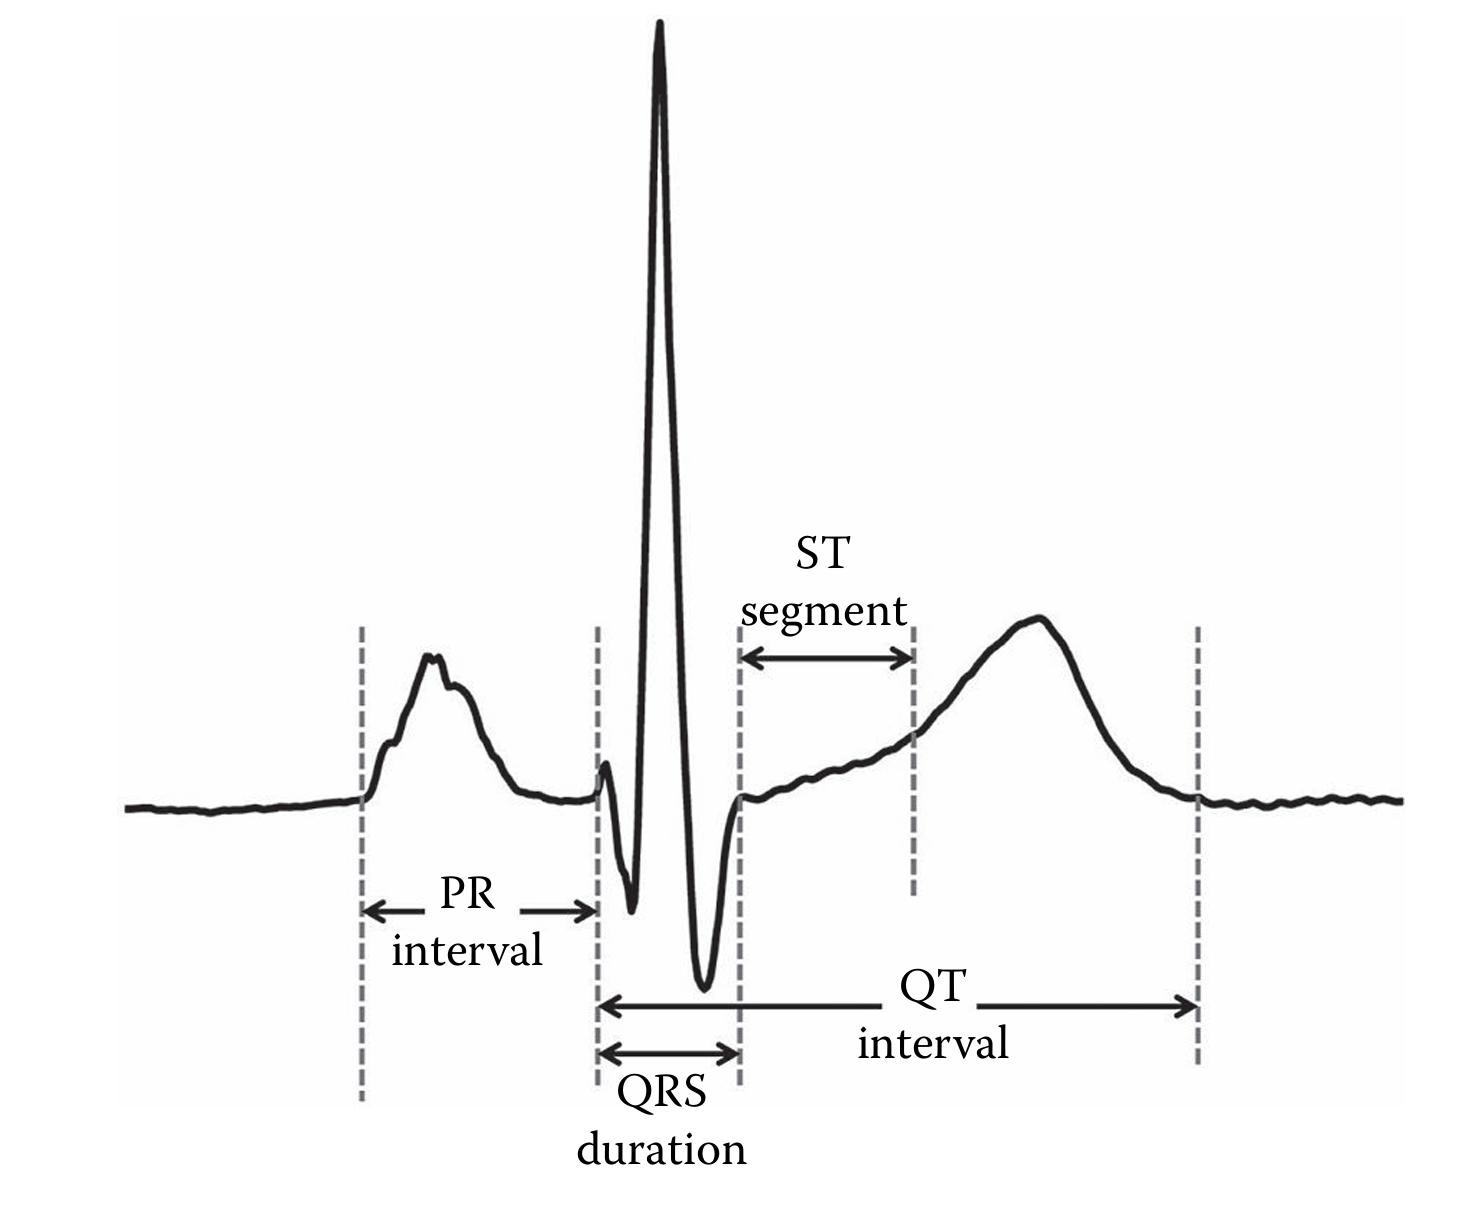
\includegraphics[width=0.6\linewidth]{assets/QRS.png}
    \caption{Ilustração dos intervalos e segmentos padrão medidos no ECG. Fonte: \cite{webster}.}
    % \label{fig:enter-label}
\end{figure}

%colocar figugra

Em condições normais de repouso, o ritmo sinusal apresenta frequência cardíaca entre 60 a 100 bpm (algumas diretrizes admitem entre 50–99 bpm) (\citeay{guyton2021fisiologia}). As medidas temporais padronizadas incluem o \textit{intervalo PR} (do início da onda P ao início do QRS), associado ao tempo de condução AV, com duração típica de 0{,}12--0{,}20~s~ (\citeay{marriott2018practical}). O \textit{intervalo QT} (do início do QRS até o fim da onda T), relacionado à duração da despolarização-repolarização ventricular, geralmente varia entre 0,35 e 0,45 s. O complexo QRS normal é estreito, durando cerca de 0{,}06--0{,}10~s, refletindo condução ventricular rápida pelas vias especializadas. Morfologicamente, a \textit{onda P} tem baixa amplitude ($\leq$0{,}25~mV) e curta duração (<0{,}12~s), enquanto o QRS tem amplitude maior ($\sim$1~mV) e a onda T possui polaridade geralmente concordante com o QRS (\citeay{brazilian_guidelines_ecg}). Esses parâmetros quantificáveis são essenciais para diferenciar padrões normais e patológicos, como bloqueios atrioventriculares, bloqueios de ramo ou prolongamentos de QT com potencial arritmogênico.

A aquisição precisa do sinal \acs{ECG} requer conformidade com especificações técnicas rigorosas, estabelecidas por normas como \textit{ANSI/AAMI EC11}, \textit{IEC 60601-2-25} e \textit{IEC 60601-2-47}. O circuito de entrada deve garantir alta rejeição de modo comum (\textit{CMRR} típico > 90 dB) e tolerância a tensões de offset nos eletrodos de até ±300 mV, já que o sinal útil está na ordem de 1 mV (AAMI, \citeyear{aamiEC11}). A largura de banda depende do propósito: aplicações diagnósticas exigem captura de frequências entre 0{,}05 Hz e 150 Hz, enquanto a monitorização ambulatorial pode operar em bandas entre 0{,}5–40 Hz para reduzir artefatos e interferências(IEC, \citeyear{iec60601}). Após amplificação e filtragem, o sinal é digitalizado com taxas de amostragem típicas entre 250 e 500 Hz, preservando a morfologia do QRS.


Em contextos clínicos, a análise eletrocardiográfica padrão baseia-se no sistema de 12 derivações, que permite a visualização da atividade elétrica cardíaca em múltiplos planos—frontal e horizontal—proporcionando uma avaliação abrangente da condução e da repolarização miocárdica. As derivações bipolares dos membros (DI, DII e DIII) e as unipolares aumentadas (aVR, aVL e aVF) compõem o plano frontal, fornecendo diferentes ângulos de observação da atividade elétrica em direção aos eletrodos dos membros. Já as derivações precordiais (V1 a V6), dispostas na parede torácica, integram o plano horizontal e são fundamentais para localizar alterações segmentares, como na identificação de infartos transmurais e bloqueios de ramo. A correta interpretação dessas 12 derivações exige compreensão da vetorização do impulso elétrico e da anatomia cardíaca, pois cada uma reflete a atividade elétrica de regiões específicas do miocárdio, sendo imprescindível para a caracterização topográfica de eventos isquêmicos, distúrbios de condução e alterações eletrolíticas. Assim, o ECG de 12 canais permanece uma ferramenta diagnóstica insubstituível, sintetizando informações morfológicas, temporais e espaciais do ciclo cardíaco com elevado grau de resolutividade clínica. (\citeay{brazilian_guidelines_ecg}; \citeay{marriott2018practical})





\section{Fundamentos da Tecnologia LoRaWAN}
\label{sec:lorawan}

A tecnologia LoRaWAN posiciona-se entre as redes de longa distância e baixa potência (\textit{Low Power Wide Area Networks} -- LPWAN), categoria concebida para conectar grande número de dispositivos que transmitem pequenos volumes de dados de forma esporádica, com ênfase em alcance e autonomia energética em detrimento da taxa de transferência. Compreender seus fundamentos é essencial para justificar as decisões de projeto adotadas neste trabalho, em especial a escolha da classe de operação e a estratégia de transmissão (Capítulo~\ref{chap:metodologia}).

\subsection{Modulação LoRa}
\label{sec:moduloLora}

Na camada física, o LoRa emprega a modulação por espalhamento espectral do tipo \textit{Chirp Spread Spectrum} (\acs{CSS}), na qual a informação é codificada em sinais cuja frequência varia continuamente ao longo do tempo (\textit{chirps}) (\citeay{loraSpec}). Essa técnica confere elevada robustez a interferências e a efeitos de propagação por múltiplos percursos (\textit{multipath}), além de permitir a recuperação de sinais com potência abaixo do nível de ruído. O principal parâmetro da modulação é o fator de espalhamento (\textit{Spreading Factor} -- SF), que varia tipicamente de 7 a 12: fatores mais altos aumentam o alcance e a sensibilidade do receptor, ao custo de maior tempo de transmissão e menor taxa de dados (\citeay{loraOverview}). Em conjunto com a largura de banda (\textit{Bandwidth} -- BW), geralmente de 125 kHz, o SF determina a taxa de transmissão efetiva e o tempo de ocupação do canal (\textit{Time on Air}).

\subsection{Arquitetura da Rede}
\label{sec:arqLora}

O LoRaWAN define a camada de controle de acesso ao meio (MAC) sobre a modulação LoRa, organizando a comunicação segundo uma topologia em estrela de estrelas (\textit{star-of-stars}). Nessa arquitetura, os dispositivos finais (\textit{end-devices}) comunicam-se por difusão com um ou mais \textit{gateways}, que atuam como pontes transparentes e encaminham os pacotes recebidos a um servidor de rede (\textit{network server}) por meio de uma conexão IP convencional. O servidor de rede é responsável por remover pacotes duplicados, validar a autenticidade dos dispositivos, gerenciar os parâmetros de transmissão e repassar os dados ao servidor de aplicação (\citeay{lorawan1}; \citeay{s23208440}). A segurança é assegurada por criptografia AES de 128 bits em dois níveis independentes — rede e aplicação —, garantindo a confidencialidade dos dados desde o dispositivo até a aplicação final.

\subsection{Classes de Operação}
\label{sec:classesLora}

A especificação LoRaWAN define três classes de operação, que estabelecem o compromisso entre latência de comunicação no sentido descendente (\textit{downlink}) e consumo de energia, conforme resume a Tabela~\ref{tab:classesLora} (\citeay{loraOverview}; \citeay{lorawan1}).

\begin{table}[h]
    \centering
    \caption{Classes de operação do protocolo LoRaWAN.}
    \begin{tabular}{l|>{\arraybackslash}m{6.5cm}|c}
        \textbf{Classe} & \textbf{Funcionamento} & \textbf{Consumo} \\ \hline
        A & Duas janelas curtas de recepção abertas somente após cada \textit{uplink}; \textit{downlink} apenas em resposta. & Mínimo \\ \hline
        B & Janelas de recepção adicionais, agendadas por \textit{beacons} sincronizados do \textit{gateway}. & Intermediário \\ \hline
        C & Janela de recepção continuamente aberta, exceto durante a transmissão; menor latência de \textit{downlink}. & Máximo \\ \hline
    \end{tabular}
    \label{tab:classesLora}
\end{table}

A Classe~A é o modo obrigatório, suportado por todos os dispositivos, e o de menor consumo energético, sendo adequado a dispositivos alimentados por bateria. Sua principal limitação reside no fato de que a recepção de mensagens descendentes só ocorre após uma transmissão ascendente, o que restringe a taxa efetiva de comunicação — característica determinante para o comportamento observado nos experimentos deste trabalho (Capítulo~\ref{chap:resultados}).

\subsection{Parâmetros de Transmissão e Limitações}
\label{sec:paramsLora}

A combinação de SF e largura de banda é abstraída em um índice de taxa de dados (\textit{Data Rate} -- DR), cuja correspondência varia conforme o plano regional de frequências. O LoRaWAN opera em bandas de frequência não licenciadas (\textit{Industrial, Scientific and Medical} -- ISM), específicas de cada região: 868 MHz na Europa, 915 MHz nas Américas — incluindo o plano AU915, adotado neste trabalho — e 433 MHz em partes da Ásia (\citeay{s23208440}). O tamanho máximo do \textit{payload} é condicionado ao DR e situa-se na faixa de poucas dezenas a poucas centenas de bytes.

A principal restrição à transmissão frequente decorre das regras de \textit{duty cycle} impostas às bandas ISM, que limitam a fração de tempo em que um dispositivo pode ocupar o canal, obrigando intervalos mínimos entre transmissões. Mecanismos como a taxa de dados adaptativa (\textit{Adaptive Data Rate} -- ADR) permitem ao servidor de rede ajustar dinamicamente o SF e a potência de transmissão de cada dispositivo, otimizando o consumo e a capacidade da rede (\citeay{performanceLoRa}). Tais limitações tornam o LoRaWAN inadequado à transmissão contínua de formas de onda de alta resolução, como o \acs{ECG} amostrado, porém plenamente eficiente para o envio de dados esparsos e de pequeno volume, como parâmetros vitais e alertas de detecção (\citeay{lorawanWaveform}; \citeay{3-lead}) — premissa que fundamenta a abordagem de processamento na borda adotada neste trabalho.



